% !TeX root = sigqdyn_tr.tex
% ================================================================
\section{The Problem}\label{sigqdyntr_problem}
% ----------------------------------------------------------------
\subsection{The Problem in Brief}\label{sigqdyntr_problem_brief}
The signal from an AQM can be subject to unnecessary \textbf{queuing delay} if it is applied to a packet during the enqueue process, so that it has to work its way through the queue before being transmitted to the line. In classical AQMs, queuing delay is configured to be of the same order of magnitude as typical propagation delays. Therefore subjecting the congestion signal to the delay of the queue will add unnecessary sloppiness to the control loop.

Even if a signal is applied to a packet as it is dequeued, it is often based on a \textbf{measurement} that has taken some time to collect. For instance, the sojourn time technique, which is becoming common for measuring the queue in modern AQMs, gives a queue delay metric that is always out of date by the amount of time the packet spent in the queue. So even if the signal is applied at dequeue, it is delayed by the time spent measuring it in the queue.

The sojourn time measured when a packet reaches the head of the queue takes no account of any change in the queue while that packet is working towards the head. Despite the queuing system holding all the information about those recent changes. So if a burst arrives, the sojourn time of packets in front of the burst will show no evidence of the queue building behind them. For instance, in \autoref{fig:sojourn-prob}a), the sojourn of the first packet of the burst takes '0' timeslots. And the sojourn time metric only fully measures the burst when the last packet of the burst reaches the head of the queue, where '9' is shown. Even though, in this case, all the packets of the burst had arrived before the packet tagged '1' was dequeued. In \S\,\ref{sec:fairer_marking} we will consider a mix of smooth and bursty traffic, then we will see how this delay attributing blame for a burst tends to shift the blame from bursty to smooth traffic.

Whenever the drain rate abruptly reduces, use of sojourn time is similarly problematic. As soon as the reduction occurs, the time that packets will take to work through the queue increases. But, the sojourn time of those packets that have already worked their way towards the head of the queue does not reflect the delay that will be experienced by the packets behind them.

Conversely, consider the queue in \autoref{fig:sojourn-prob}b) that has been stable then the data flow ends abruptly, so that no further packets arrive. Then, even when the last packet to arrive is about to be dequeued from the head of the queue, its sojourn time still measures the stable queue delay when it arrived, because that's how long it took to drain the queue. If sojourn alone were used for marking and dropping, there would be no externally visible evidence of the now empty queue behind the last packet until traffic started again.

Implementations of AQMs that use sojourn time sometimes include code to deal with certain exceptional cases (such as an empty queue). But this memo proposes simple techniques to cut out the root cause of that measurement delay in all cases; by using all the information available in the queue at the point that a packet is dequeued. At dequeue there is very little time for additional processing, so considerable attention has had to be paid to minimizing execution time as well.

% ----------------------------------------------------------------
\subsection{The Time to Measure the Service Time of a Queue}\label{sec:svc_time}

In around 2012, it became recognized that one of the main problems with AQMs was the sensitivy of their configuration to changing environments. For example:
\begin{itemize}
	\item access links often change their rate when modems retrain in response to interference. 
	\item a queue can be part of a scheduling hierarchy and traffic in higher priority queues varies the capacity left for a lower priority queue, rapidly varying the drain rate that the AQM experiences.
	\item the rate of typical WiFi links varies rapidly over time~\cite{McGregor10:Minstrel_TR}.
\end{itemize}

The CoDel algorithm~\cite{Nichols12:CoDel} proposed to solve this problem by measuring the queue in units of time, rather than bytes. This made the configuration of the thresholds in the algorithm independent of the drain rate.

Actually, as far back as 2002, 
Kwon and Fahmy~\cite{Kwon02:Load_v_Queue_AQM} had advised that the queue should 
be measured in units of time. Also, in 2003, S{\aa}gfors \emph{et al} had 
modified the Packet Discard Prevention Counter (PDPC+~\cite{Sagfors03:PDPC_vary}) 
algorithm by converting queue length to queuing delay to cope with the varying 
link rate of 3G wireless networks. PDCP still measured the queue in bytes, but then converted the result to time by dividing by the link rate, which it measured over a brief interval. 

CoDel proposed an elegant way to measure the service time of the queue by adding a timestamp to each packet's internal metadata on enqueue. Then at dequeue, it subtracted this timestamp from the system time. The authors called the result the sojourn time of the packet. It was also pointed out that this sojourn time could be measured over an arbitrarily complex structure of queues, even across distributed input and output processors.

Because PIE~\cite{Pan13:PIE} was initially designed for implementation using existing hardware, it did not measure the service time of the queue directly using the time-stamping approach of CoDel.
Instead, like PDPC, it converted queue length to queuing delay using a regularly updated 
estimate of the link rate, measured over a set amount of packets. When there were insufficient packets in the queue to measure the link rate or the rate was varying rapidly, PIE's estimate of the link rate became stale. So in later specifications of PIE~\cite{Pan17:PIE}, it recommended the sojourn approach of CoDel that had originally been designed for software implementation.

The queue length (in bytes or an equivalent unit), also called the backlog, can be measured instantaneously when a packet is enqueued or when it is dequeued. In contrast, it takes a sojourn time to measure sojourn time (which can only be measured as a packet is dequeued). So measuring sojourn time inherently introduces delay into the control path.

To minimize delay, the signal should be applied at dequeue. However, in some hardware pipelines the process of preparing link layer frames, including potential encryption, compression and framing, is already in progress by the time a packet is dequeued. So it is too late to mark or drop a packet. This is one reason that PIE initially applied the congestion signal when it enqueued a packet. That is, it probabilistically dropped (or ECN-marked) the packet when it enqueued it. This signal then worked its way through the queue before being transmitted, adding a sojourn time of delay to the signal. This is still the case for DOCSIS PIE, but software variants of PIE now apply marking or dropping at dequeue. 

The matrix in \autoref{tab:added-delay} shows the delay added to the signal by various techniques for measuring queue delay that will be introduced later (horizontal) and the two choices for where to apply the signal (vertical). It uses the following terminology: \(t_r\) is the duration used to sample the drain rate and \(t_s\) is the sojourn time. 
\begin{table}[h]
\begin{center}
\begin{tabular}{p{0.17\columnwidth}|C{0.16\columnwidth}*{2}{C{0.2\columnwidth}}}
\multirow{3}{0.17\columnwidth}
{Where signal is applied}
			& \multicolumn{3}{c}{Technique to measure queue delay}\\
			& \multirow{2}{0.17\columnwidth}
			  {Sojourn Time}
			            & \multicolumn{2}{C{0.5\columnwidth}}
			              {Expected Service Time}\\
                          \cline{3-4}
			&			& Time-Based Backlog&  Scaled Sojourn Time\\\hline 
	at enq  & \(2t_s\)	& \(t_r + t_s\)	& \(3t_s/2\)\\
	at deq  & \(t_s\)	& \(t_r\)			& \(t_s/2\)
\end{tabular}
\caption{Delay added to congestion signal by three different measurement techniques}%
\label{tab:added-delay}
\end{center}
\end{table}

The centre column shows the effective delay added by the simple `Time-Based Backlog' technique proposed in \S\,\ref{sec:time-based_backlog}. It also applies to the variant of that technique called `Size-Adjusted Threshold' in \S\,\ref{sec:time-adj_thresh}. The right hand column shows the delay of a technique called `Scaled Sojourn Time' introduced in \S\,\ref{sec:scaled_svc_time}, which can be used where the ability of sojourn time to measure delay across a complex set of queues is required. Nonetheless, for a simple software queue, the time-based backlog is preferable, because it always adds minimal measurement delay.

It can be clearly seen that applying a signal at enqueue adds \(t_s\) to the signal delay.
So applying the signal at enqueue would only be appropriate if it were not possible to mark (or drop) a packet at the head of the queue, e.g.\ due to implementation or timing constraints.

% ----------------------------------------------------------------
\subsection{The Blame Shifting Problem}\label{sec:fairer_marking}

When the Random Early Detection (RED) AQM algorithm was first proposed, fairness was one evaluation factor~\cite[\S\,8]{Floyd93:RED}. Fairness in the context of marking was defined as ``the fraction of marked packets for each connection is roughly proportional to that connection’s share of the bandwidth''. 

Such fairness would be sufficient if all flows were long lived and smooth, but they are not.  Wischik~\cite{Wischik99:Mark_Fairly} contrives a simple two-flow scenario to demonstrate how RED can shift nearly all the marking from a burst in one flow onto a smoother flow that continues after the burst. %In this scenario one flow usually sends at a lower rate than the other, but then suddenly causes congestion by sending faster for a brief period before returning to its lower rate. The queue smoothing algorithm within the RED AQM delays nearly all the congestion marking until after the congested period ends, when most arrivals are from the constant flow. 

Classical AQMs like RED or more recent designs such as CoDel or PIE are designed to filter out variations in the queue over a likely maximum round trip. So they inherently introduce smoothing delay of about 100--200\,ms prior to signalling congestion, which is far too long to be able to mark packet bursts correctly. More recently, the importance of immediate congestion signalling has been recognized in approaches such as Data Center TCP (DCTCP~\cite{Alizadeh10:DCTCP}) and Low Latency Low Loss Scalable throughput (L4S~\cite{Briscoe16a:l4s-arch_ID}), where the job of smoothing out variations is shifted from the AQM to the sender.

Marking fairness has been termed `shadow pricing'~\cite{Kelly98:Shadow_prices_prop_fair} or `cost fairness'~\cite{Briscoe06g:Rate_fair_Dis}, because it ensures the cost or harm to others of each user's behaviour can be measured. Note that marking fairness is an important mechanism requirement for all AQMs and should not be confused with flow-rate `fairness', which is an arbitrary policy choice concerning allocation of benefits at any instant (which is why `fairness' is placed in quotes in this latter case)\footnote{The RED paper went on to explain that ``RED gateways do not attempt to ensure that each connection receives the same fraction of the total throughput''.}. 

This section introduces fairness problems when sojourn time is used to mark flows with different degrees of burstiness. Then it uses a worked example to give better intuition for how to make marking fairer. The question of what marking would actually be fair for different degrees of burstiness is deferred to a later discussion section (\S\,\ref{sec:marking_fairness_discuss}). 

Nonetheless, we will now demonstrate that even the delay spent measuring sojourn time is enough to cause immediate marking to miss packet bursts, and hit smoother flows instead. Although we cannot yet say exactly what is fair, we can recognize this shift of blame, when one marking approach is significantly less fair than another.

\begin{figure}[h]
	\centering
	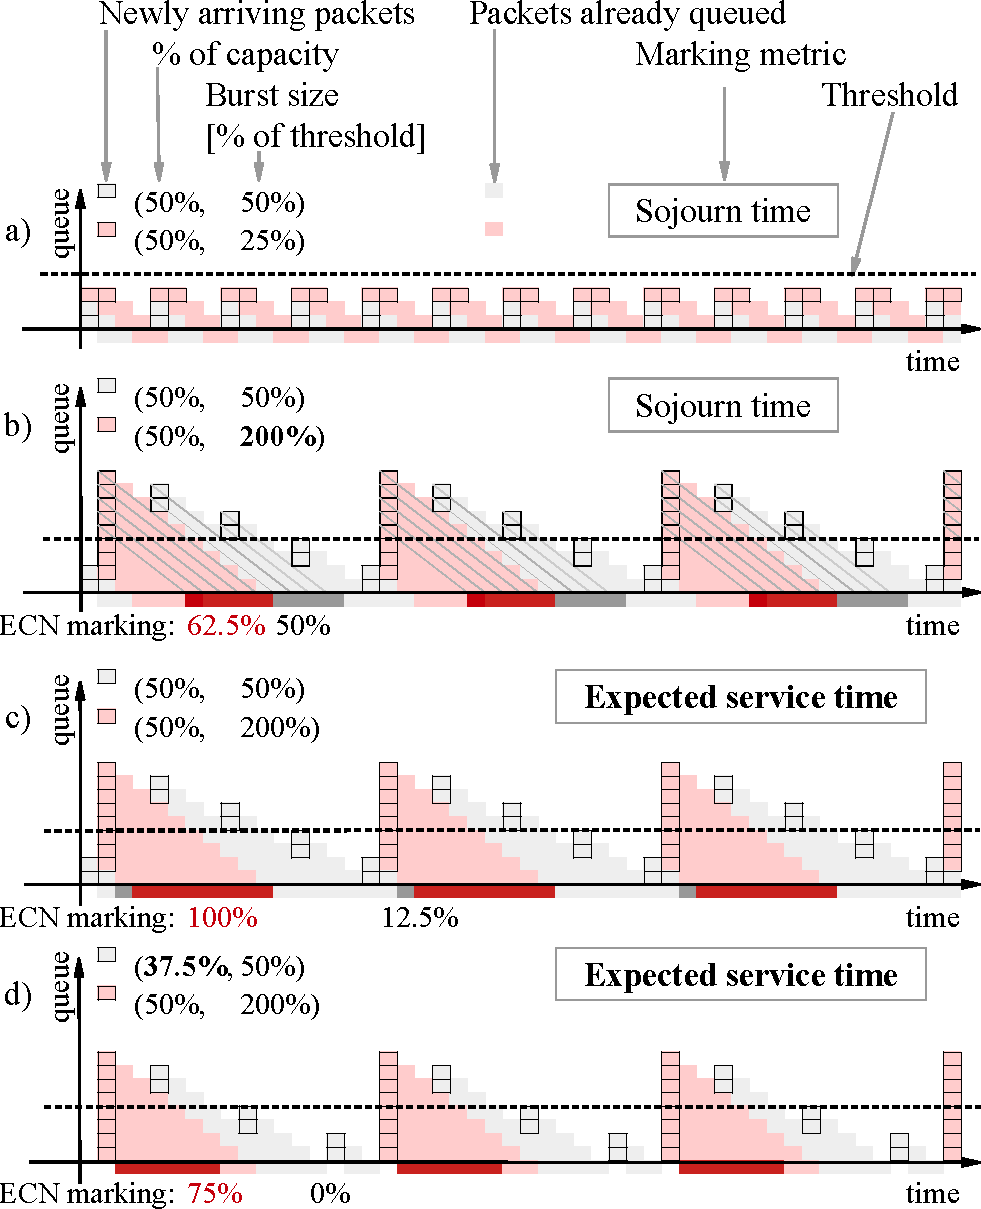
\includegraphics[width=\columnwidth]{marking-fairness5050}
	\caption{The Blame Shifting Problem and a way to solve it by replacing Sojourn Time with an Expected Service Time (EST) metric. %A time-series of the queue in a progression of simplified scenarios (a--d) is shown, with one change at a time, each highlighted in bold. a) is the baseline with grey:pink average arrival ratio of 50:50 and both with low burstiness. In both b) \& c) the two flows rates continue to average 50:50 but the pink flow arrives in larger, less frequent bursts. In c) the traffic is the same as b), but the marking algorithm is different; the dark red and dark grey packets below each x-axis indicate congestion-marked packets. Scenario d) illustrates the grey flow starting to respond to the congestion marking, while the pink flow remains unresponsive
	ECN marking (shown as darker packets under each x-axis) ought to indicate which packets are most to blame for queuing. But in (b) uing a sojourn metric, the pink bursts cause grey packets to attract nearly as much marking as pink. In (c) \& (d), the expected service time metric better ensures that ECN marking reflects the blame for any queuing. See text for full explanation and commentary.}\label{fig:marking-fairness5050}
\end{figure}

\autoref{fig:marking-fairness5050} shows how a packet queue behaves in a progression of four scenarios reduced to their essentials by using equal-sized packets; one timeslot per delivered packet; a constant rate link; a step ECN marking threshold (the dashed horizontal line); and high link utilization; but without modelling the interaction with the sender's congestion control. 

In the first three scenarios (a--c), two flows (grey and pink) fully utilize the link, consuming 50\% each. Newly arriving packets have a border while packets already queued do not, as shown in the legend above the top scenario. In all four scenarios, the grey packets arrive in small bursts, each the size of half the queue delay threshold. Other aspects of the traffic and marking algorithm change over the progression of scenarios, as highlighted in bold in each row of the figure and described below:
\begin{enumerate}[nosep, label=\alph*)]
	\item This is the baseline case to show that the pink flow can fill the capacity left by the grey flow without exceeding the threshold, as long as it keeps its bursts small enough (in this case just 25\% of the threshold, making at most 75\% if a pink burst were to coincide with a grey one). 
	\item In this case, each burst from the pink flow occupies 200\% not 25\% of the threshold in the buffer. The average rate of both flows is unchanged, so the link is still 100\% utilized, and the grey flow still arrives in the same pattern of small bursts. So, in the time the pink burst takes to drain, some of the smaller grey bursts back up behind it and, while they are draining, more small grey bursts accumulate. So the queue only finally empties just as the cycle starts to repeat with the arrival of the next pink burst.
	\item The arrivals in this scenario are identical to (b), but sojourn-based queue measurement is replaced with expected service time (EST---described below).
	\item In this last case, we attempt to represent the grey flow starting to respond to the ECN marking in (c), while the pink flow remains unresponsive at 50\% of the link and still arriving in large bursts twice the depth of the threshold. The flow rate of the grey flow reduces from 50\% to 37.5\% of the link or \(\sfrac{3}{4}\) of the rate of the pink flow.
\end{enumerate}

The ECN marking metric is written in the box above each scenario:
\begin{description}
	\item[Sojourn time:] In scenario b) in \autoref{fig:marking-fairness5050}, each diagonal darker line traces the sojourn through the queue of those packets that arrive when the queue is above the threshold. The service time or sojourn time of these packets will have exceeded the threshold so they will be marked on departure (shown under the axis as darker coloured packets). The proportion of marked packets of each colour is written under that.

	\item[Expected Service Time:] In scenarios c) or d) there are no diagonal lines, because, rather than measuring the delay of the packet itself, EST measures the delay that a packet causes to others. Various ways in which EST has been or could be implemented will be given in \S\,\ref{sec:exp_svc_time}, but briefly, instead of marking a packet based on the queue in front of it, EST estimates the queue delay \textit{behind} a packet at the instant it departs. In the schematic, EST marks departing packets (darker coloured) if the vertical depth of the queue in the timeslot just before departure exceeds the threshold.\footnote{The EST algorithm uses queue delay, but in this simplified illustration queue depth represents delay because the drain rate is constant.}
\end{description}

In this second pass, we comment on the ECN marking outcome from each scenario:
\begin{enumerate}[nosep, label=\alph*)]
	\item There is no ECN marking in this baseline case (whatever the metric).
	\item The sojourn times of 5/8 of the packets at the tail of the pink burst exceed the threshold. So the sojourn-based AQM marks 62.5\% of the pink packets at dequeue. Because grey packets back up, first behind the pink burst then behind themselves, their sojourn times exceed the threshold for the first 50\% of the grey packets between each pair of pink bursts. Thus, the marking probability of the pink flow is only slightly greater than the grey, even though the pink flow's excessive burstiness is largely to blame for the queue exceeding the threshold.\footnote{Indeed, if each pink burst had happened to arrive one timeslot later, its marking would have been the same as the grey.}
	\item Here the evolution of the queue is identical to scenario (b), but marking is based on the `Expected service time' (EST) metric described above. This increases the pink marking probability from 62.5\% to 100\%, because every pink packet in the burst has caused a queue to back up behind it. In contrast, EST only marks one grey packet in each pink burst cycle --- the one that the pink burst happens to arrive behind. Thus grey marking reduces to 12.5\%, compared to 50\% with the sojourn metric.
	\item As the load from responsive grey traffic falls a little, after each unresponsive pink burst the queue falls below the threshold considerably sooner. This completely removes all grey marking, thus rewarding the grey flow for its responsiveness without too much under-utilization. The grey flow's response also reduces pink marking, but only to 75\%.
\end{enumerate}

The wider space of scenarios like this has been investigated by varying the relative shares and relative burst sizes between flows (see \S\,\ref{sec:marking_fairness_discuss}). Although the difference between the sojourn and expected service time metrics is sometimes less dramatic and sometimes more, the following intuition is generally true for all scenarios.

A smoother flow has smaller but more frequent arrival events compared to a bursty flow. So, although the bursty flow might happen to back up behind one of the smaller bursts of the smoother flow, multiple arrival events of the smoother flow will back up behind the larger burst. Therefore proportionately more of a bursty flow will be near the head of the buffer, and the packets of a smoother flow will be more likely to be occupying the tail. Figures \ref{fig:marking-fairness8020} \& \ref{fig:marking-fairness8020_4} illustrate this general point with a couple of different example traffic models.

\begin{figure}[h]
	\centering
	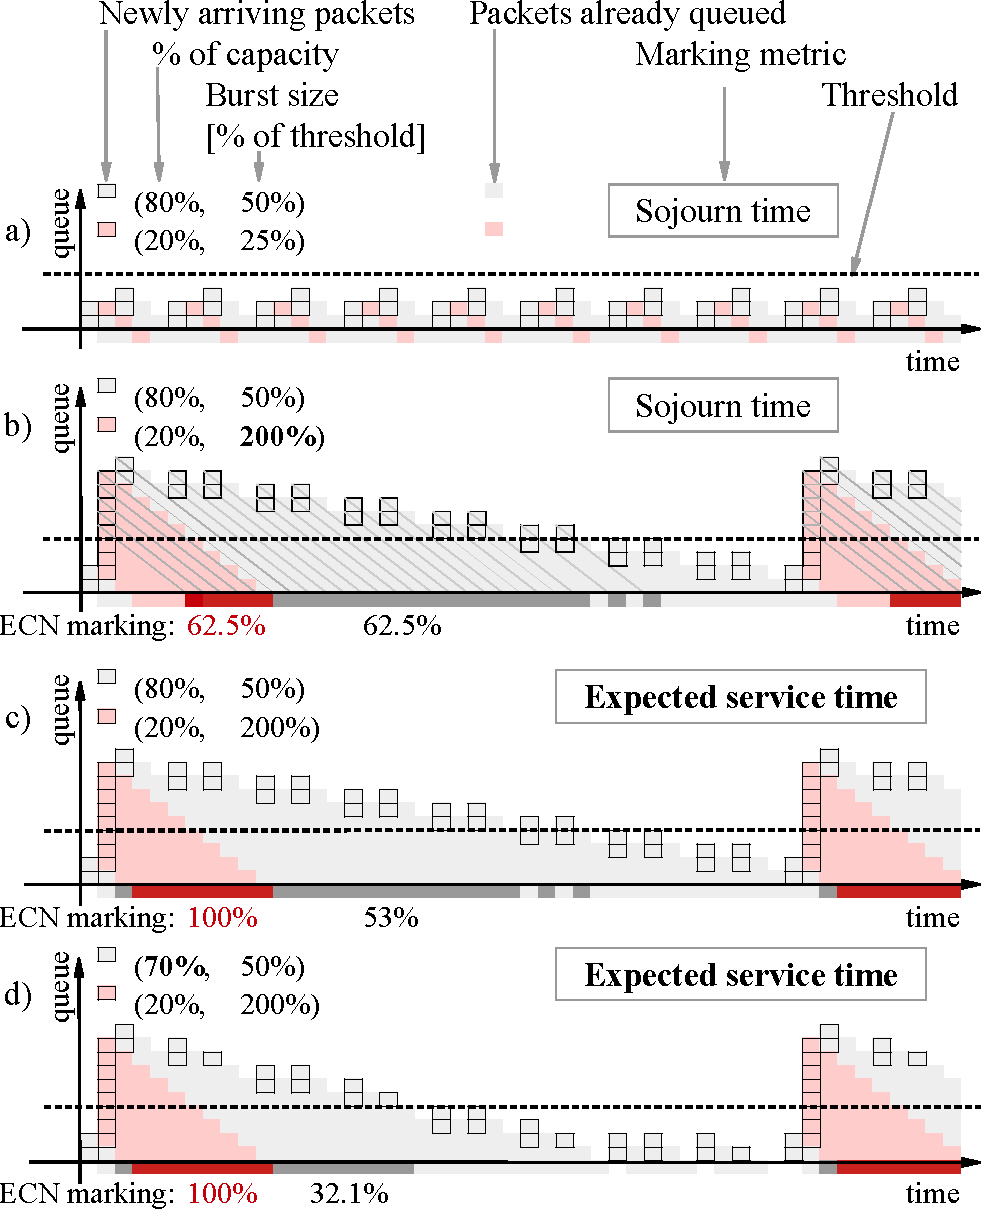
\includegraphics[width=\columnwidth]{marking-fairness8020}
	\caption{The Blame Shifting Problem with a minority of bursty unresponsive traffic using the sojourn metric (pink), and a solution using an EST metric.}\label{fig:marking-fairness8020}
\end{figure}

The grey:pink ratio in \autoref{fig:marking-fairness8020} is 80:20 rather than 50:50, but other aspects like burst sizes are the same as in \autoref{fig:marking-fairness5050}. \autoref{fig:marking-fairness8020}b) shows that the sojourn metric still allows the pink bursts to shift about half the blame for marking onto the grey flow. In contrast, EST marking (\autoref{fig:marking-fairness8020}c) again subjects the pink flow to the maximum possible blame (100\% marking). But this time the grey flow still attracts a little over 50\% marking, which reflects the greater proportion of the link that it consumes. 

Nonetheless, a slight grey reduction to \(\sfrac{7}{8}\) of its previous rate (\autoref{fig:marking-fairness8020}d), reduces its marking to just over 30\%, while still subjecting the bursty pink flow to 100\% marking. With sojourn marking, the same reduction by the grey flow would have reduced its marking to 37.5\% (not shown). So by shifting less blame to the grey flow, EST will lead to less underutilization than sojourn in steady state. EST also continues to attribute a higher degree of blame to the unresponsive pink bursts (100\% marking). Also, a congestion policer driven by EST marking would discriminate between the flows better than if driven by sojourn.

\begin{figure}[h]
	\centering
	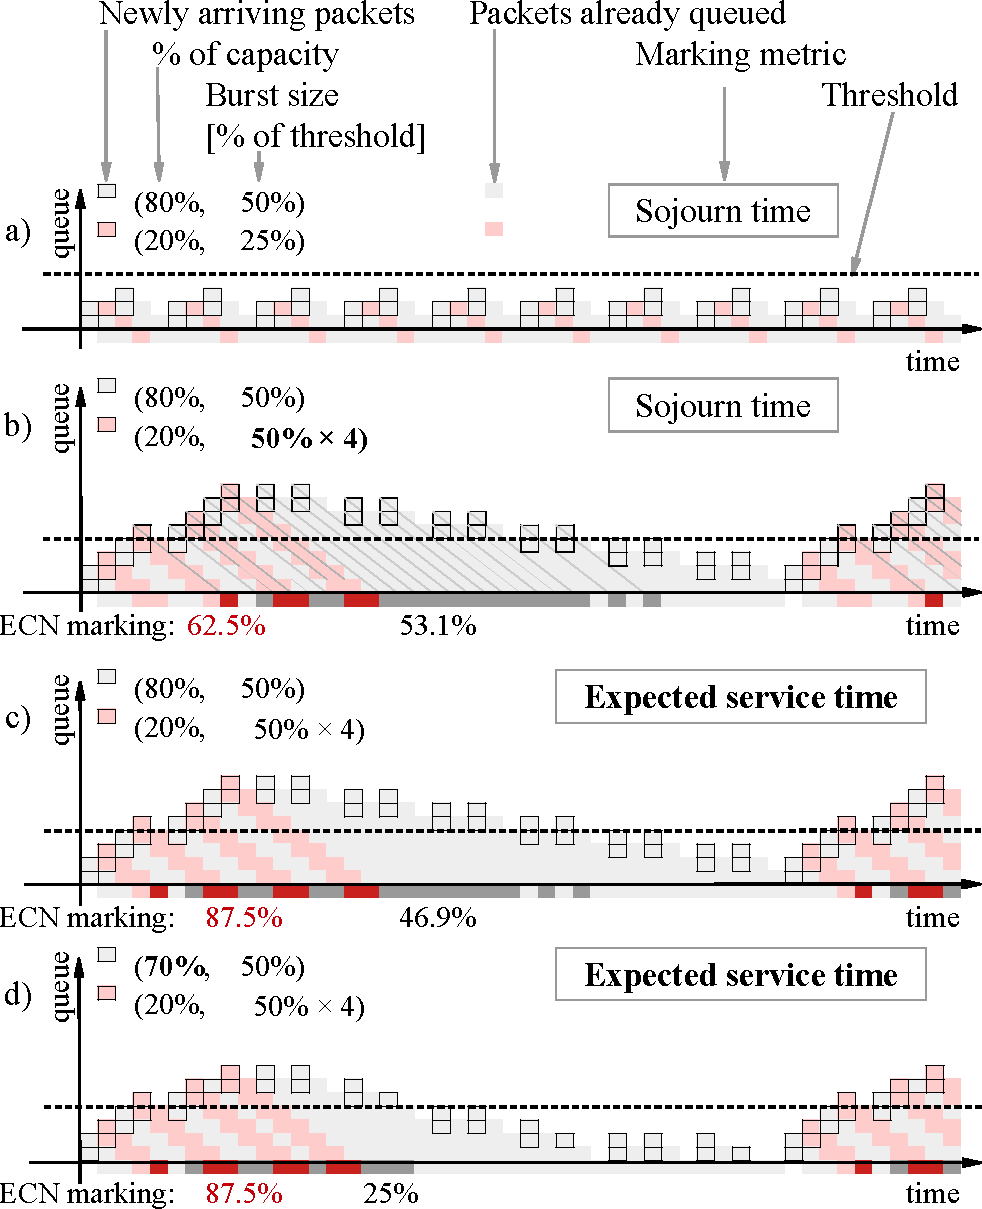
\includegraphics[width=\columnwidth]{marking-fairness8020_4}
	\caption{The Blame Shifting Problem with the sojourn metric using two flows of equal burstiness; one continuous (grey); the other intermittent (pink). And a solution using an EST metric.}\label{fig:marking-fairness8020_4}
\end{figure}

The traffic model in \autoref{fig:marking-fairness8020_4} is similar to the grey:pink 80:20 case in \autoref{fig:marking-fairness8020} except the pink flow divides the one burst into four smaller bursts of the same size (50\% of the threshold) and paced at the same rate as the continual grey bursts. Sojourn-based marking results in the same 62.5\% pink marking probability as in Figures \ref{fig:marking-fairness5050} \& \ref{fig:marking-fairness5050}. But grey marking is slightly lower than either. This is because sojourn-based marking reflects `harm to self due to others packets' and there is less pink burstiness. In contrast, with EST (\autoref{fig:marking-fairness8020_4}c), pink marking is higher and grey is lower, but the improvement is not as pronounced as in \autoref{fig:marking-fairness8020}c). In \autoref{fig:marking-fairness8020}d), the grey traffic reduces its own marking considerably by reduces its average pacing rate a little, but without affording any benefit to the unresponsive pink traffic. 

It may seem wrong that EST marks pink traffic more than grey, when pink paces at the same rate as grey but for less of the time. However, it is only the proportion of pink marking that is greater. In \autoref{fig:marking-fairness8020_4}c) there are four times as many grey packets as pink. So, even though pink marking approaches double the proportion of grey, the absolute number of pink markings is less then half that of grey. While the pink flow is active, the sum of pink and grey exceeds the link capacity, so EST `punishes' both equally. But then EST stops marking the rest of the grey traffic as a reward for allowing the queue to recover by underutilizing the link.

So far, on the limited evidence of a few simple cases, we can draw the interim conclusion that marking the head packet when there is an excessive backlog behind it is likely to lead to fairer marking than marking the head packet because it experienced a backlog in front of it that held up its own sojourn through the queue. 

% ----------------------------------------------------------------
\subsection{Implications of Unfair Marking}\label{sec:effects_unfair_marking}

\paragraph{Blame shifting with bursty traffic:} The section ``Underutilization with Bursty Traffic'' of Heist and Morton's write-up \cite{Heist20:L4S_tests} injects large bursts of unresponsive traffic into a queue that applies immediate ECN marking above a shallow threshold based on the sojourn metric. When there is also smoothly paced traffic in the same queue, the bursts cause the AQM to focus more ECN markings onto the smooth traffic, and less on the bursts. Thus, using the sojourn metric allows bursty traffic to shift the blame for the queuing it causes onto smooth traffic.

This effect can be exploited to cause smoother traffic to yield more to bursty traffic. If the bursty traffic is also unresponsive itself (as it was in \cite{Heist20:L4S_tests}), it causes the smooth traffic to significantly underutilize the link. Thus, it is important to ensure that ECN marking reflects the blame for any queuing (\S\,\ref{sec:marking_fairness_definition} discusses how to quantify the apportionment of blame objectively).

The section ``Underutilization with Bursty Links'' in the same online collection of tests~\cite{Heist20:L4S_tests} shows a similar effect. When the traffic transmitted by a smooth link (e.g.\ fixed Ethernet) is mixed with traffic that has traversed a bursty link (e.g.\ WiFi), the bursty traffic causes a sojourn-based immediate AQM to shift its marking onto the smooth traffic.

\paragraph{Perverting congestion policing:} A common technique in traffic policing is to identify misbehaving traffic by the disproportionate amount of congestion marking that an AQM applies to it, as first proposed by Floyd and Fall~\cite{Floyd99:Penalty_box}. Therefore, if an AQM fails to subject bursty traffic to a fair degree of marking, it will allow bursty traffic both to evade policing and to fool the policer into punishing smoother traffic instead.\footnote{See \S\,\ref{sec:qprot_marking_fairness} for a potential efficiency improvement to queue protection based on EST marking.}

\paragraph{Late-comer Disadvantage:} TCP Segmentation Offload (TSO) in Linux (and possibly other OSs) groups a set of packet into a back-to-back aggregate or burst and calculates the maximum packets in a burst from the current pacing rate of the flow (in pkt/s):
\[\mathrm{max\_burst} = \mathrm{pacing\_rate}\times \frac{\mathrm{MAX\_BURST\_DELAY}}{\mathrm{MTU\_BITS}}.\]
The flow's pacing rate is upper bounded by the link rate, so this ensures that the burst will not cause more than MAX\_BURST\_DELAY of queuing delay at the bottleneck. However, when a new flow starts, its pacing rate is typically well below the link rate and well below the pacing rate of any flows already established over the bottleneck link. Therefore new Linux flows consist of smaller bursts while established Linux flows consist of larger bursts. 

If an AQM at the bottleneck is based on sojourn time and therefore marks larger bursts less than smaller bursts, new flows will attract a higher congestion marking probability than established flows. Then as a new flow tries to displace an established flow, it will tend to reach a point of local equilibrium before it has reached the same rate as the established flow. Thus sojourn marking can lead to a late-comer disadvantage.

\bob{Add figures from Joakim's paper}.

% ----------------------------------------------------------------
\subsection{Blame Shifting and Per-Flow Queueing}\label{sec:fq_blame_shifting}

\begin{figure}[h]
	\centering
	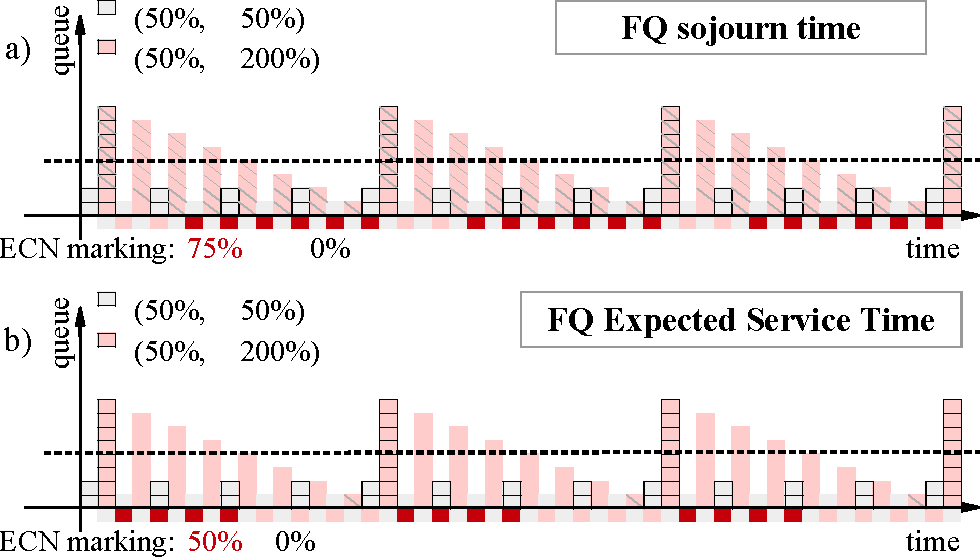
\includegraphics[width=\columnwidth]{fq-marking-fairness5050}
	\caption{Per-flow queuing (FQ) provides isolation for the grey flow from the pink bursts in the simple case of 50:50 capacity shares. Each timeslot shows only the flow-queue being served in that slot. Note that the visualization of the marking threshold is no longer useful, because the height of each queue no longer represents its delay when more than one queue is being served.}\label{fig:fq-marking-fairness5050}
\end{figure}

Heist and Morton \cite{Heist20:L4S_tests} suggest that per-flow queuing (FQ) would probably provide isolation for smooth flows from bursts. This could be true in some cases, such as the case with a more bursty pink flow sharing capacity 50:50 with a smoother flow, as shown in \autoref{fig:fq-marking-fairness5050}. Here, irrespective of whether marking is sojourn or EST-based, 75\% is focused on the pink bursts, and none on the grey flow.

\begin{figure}[h]
	\centering
	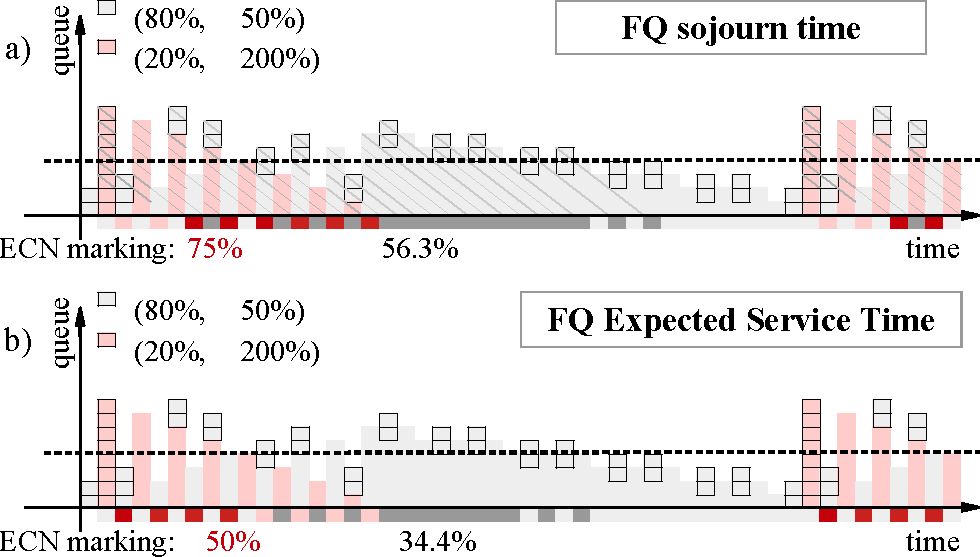
\includegraphics[width=\columnwidth]{fq-marking-fairness8020}
	\caption{FQ does not isolate the smooth grey flow from the pink bursts when their capacity shares are 80:20. FQ paces the burst better than a FIFO, but it still makes the grey flow queue up behind the burst, which it would not have done if the pink flow had arrived evenly paced. EST-based marking (b) shifts somewhat less blame onto the smooth grey flow than sojourn (a).}\label{fig:fq-marking-fairness8020}
\end{figure}

However, Figures \ref{fig:fq-marking-fairness8020} \& \ref{fig:fq-marking-fairness8020_4} show that isolation between flows breaks down for the 80:20 traffic models introduced earlier in Figures \ref{fig:marking-fairness8020} \& \ref{fig:marking-fairness8020_4}. Note here that, when grey packets arrive in a timeslot when pink packets are being served, they are shown queuing behind the pink queue (to show the slot when their sojourn timer starts), but they are then shifted into the correct queue in the next slot.

\autoref{fig:fq-marking-fairness8020}a) illustrates that this is because the scheduler serves the grey flow more slowly until it has delivered the whole of the pink burst. So the grey flow queues up and the sojourn-based AQM marks about 56\% of the grey packets, even though it would have marked zero grey if the pink flow had also been smoothly paced.

EST (\autoref{fig:fq-marking-fairness8020}b) marks the grey flow slightly less than sojourn (50\% compared to 56\%). If, as before, grey reduces its rate from 80\% to 70\% of capacity  (\autoref{fig:fq-marking-fairness8020}c), EST reduces grey marking considerably to 28.6\%. We assume that the EST marking approach for FQ introduced in \S\,\ref{sec:fq_delay_metric} is applied.

In all three cases (a--c), grey marking with FQ is a little lower than in the equivalent FIFO case in \autoref{fig:marking-fairness8020}, because of FQ's ability to pace the burst. In contrast, pink marking is much less consistently related to the equivalent FIFO cases; with FQ marking is 75\% in all three cases, whereas with a FIFO it is lower (62.5\%) with sojourn marking and much higher (100\%) in both EST cases. This is because FQ isolates the pink burst from whatever the grey flow does, and a burst on its own is marked the same whether based on sojourn or EST.

\begin{figure}
	\centering
	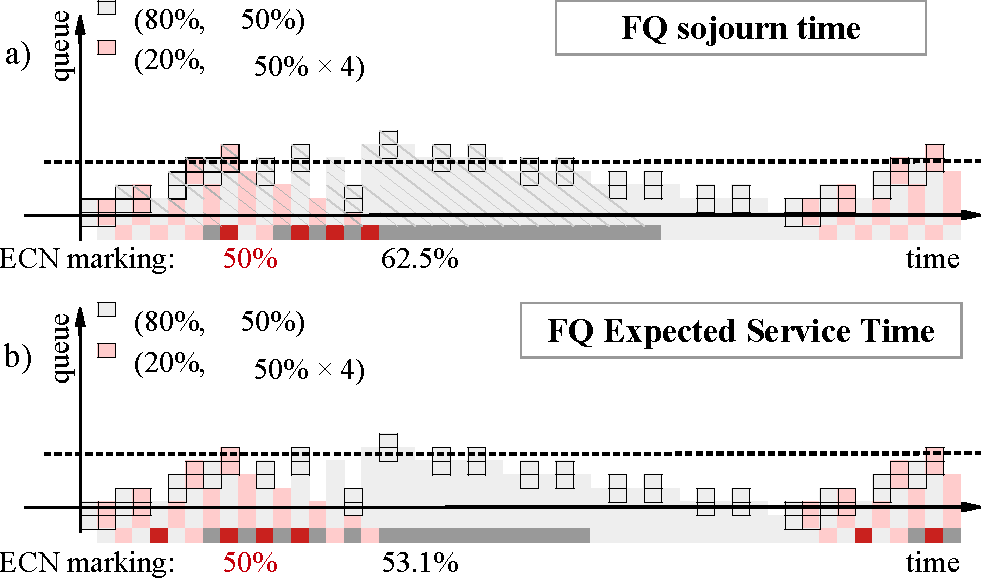
\includegraphics[width=\columnwidth]{fq-marking-fairness8020_4}
	\caption{FQ's (lack of) isolation of the grey flow from the pink is unchanged, even if the pink flow paces its burst at the same rate as the grey, but for a quarter of the time.}\label{fig:fq-marking-fairness8020_4}
\end{figure}

To complete the comparison, \autoref{fig:fq-marking-fairness8020_4} shows how FQ handles the case where the pink flow is paced at the same rate as the grey, but for only a quarter of the time. Still FQ does not isolate the grey flow from this much milder form of pink burstiness. Indeed, the grey queue and its marking is identical to the case where the pink burst all arrives in one timeslot. Nonetheless, pink marking is reduced to 50\%, which remains unchanged irrespective of the metric and irrespective of whether the grey flow reduces its rate.
